\documentclass[journal=dme,manuscript=article,11pt]{article}

\usepackage[utf8]{inputenc}
\usepackage[margin=1.0in]{geometry}
\usepackage{amsmath,amssymb,amsfonts,amsthm}
\usepackage{graphicx}
\usepackage{booktabs}
\usepackage{cite}
\usepackage{url}
\usepackage{microtype}
\usepackage{lineno}
\usepackage{setspace}
\usepackage{caption}
\usepackage{subcaption}
\usepackage{float}
\usepackage[colorlinks=true,linkcolor=blue,citecolor=blue,urlcolor=blue]{hyperref}

% Theorem environments
\newtheorem{theorem}{Theorem}
\newtheorem{lemma}{Lemma}
\newtheorem{definition}{Definition}
\newtheorem{corollary}{Corollary}
\newtheorem{proposition}{Proposition}

% Line numbering for review
\linenumbers
\onehalfspacing

\title{\textbf{Topologically Exact 3D/2D Line and Ray Clipping for Distributed CT and MRI Volume Computing: The Analytical Phase-Compensated Bresenham Algorithm}}

\author{
    \textbf{Hemanth Manchabale Papachappa}\thanks{Corresponding Author. E-mail: \texttt{hemathmpkumar123@gmail.com}; ORCID: \href{https://orcid.org/0009-0007-1398-9451}{0009-0007-1398-9451}}\\
    \textit{Independent Researcher, Seattle, Washington, USA}
}

\date{\today}

\begin{document}

\maketitle

\vspace{-0.5cm}
\begin{abstract}
Distributed forward projection and volumetric ray casting in high-resolution Computed Tomography (CT) and Magnetic Resonance Imaging (MRI) require partitioning large voxel grids across distributed GPUs, MPI ranks, or tiled cache blocks. Prevailing volumetric pipelines decouple continuous ray clipping from discrete rasterization: continuous rays are clipped against sub-volume bounding boxes, and the resulting boundary intersections are rounded to grid coordinates to reseed standard Bresenham steppers. In this paper, we demonstrate that this decoupled approach resets fractional error accumulators to zero, creating a systematic phase shift that breaks 26-voxel connectivity and corrupts traversal paths across more than 99.7\% of boundary-crossing rays. In tomographic reconstruction, this defect generates line-integral attenuation errors reaching up to 15.9\,cm$^{-1}$, producing prominent boundary streak and ring artifacts that impair iterative algebraic convergence. To address this problem, we present the \emph{Analytical Phase-Compensated Bresenham} (AP-Bresenham) algorithm. By deriving the closed-form Diophantine dynamics of 3D digital lines, AP-Bresenham evaluates exact integer entry coordinates and historical error accumulator states at any sub-volume boundary in $O(1)$ time, eliminating the need for inter-node communication or ghost-cell buffers. Evaluated across synthetic 3D head phantoms and clinical abdominal CT and brain MRI patient scans partitioned into up to 512 distributed sub-volumes, AP-Bresenham completely eliminates boundary seam gaps, preserves exact Radon line integrals ($\mathrm{RMSE} = 0.0000$, $\mathrm{PSNR} = \infty$), and achieves a 1.2$\times$--1.6$\times$ setup speedup over conventional floating-point clippers.
\end{abstract}

\vspace{0.2cm}
\noindent \textbf{Keywords:} computed tomography, magnetic resonance imaging, volume ray casting, discrete tomography, distributed computing, bresenham algorithm, diophantine dynamics, image reconstruction

\newpage

% ==============================================================================
% 1. INTRODUCTION
% ==============================================================================
\section{Introduction}
\label{sec:intro}

High-resolution 3D volumetric imaging---including Computed Tomography (CT), Magnetic Resonance Imaging (MRI), and multi-modality PET/CT systems---forms the backbone of modern diagnostic medicine, radiotherapy target delineation, and computer-assisted surgical navigation.\cite{feldkamp1984practical,siddon1985fast,jacobs1998fast,long2010separable,kim2024heterogeneous,zhang2023distributed,wang2025distributed,liu2026ultra} At the core of high-fidelity iterative reconstruction frameworks (e.g., Algebraic Reconstruction Techniques such as SART and SIRT, as well as statistical Maximum Likelihood Expectation Maximization [MLEM]) is the repeated evaluation of radiological line integrals:
\begin{equation}
    \label{eq:radon_integral}
    p(L) = \int_L \mu(\mathbf{x}) \, ds \approx \sum_{v \in \mathcal{V}(L)} \mu(v) \, \Delta s(v),
\end{equation}
where $L$ denotes the line-of-response (LOR) or X-ray trajectory, $\mu(\mathbf{x})$ denotes the spatial distribution of the linear attenuation coefficient (or proton spin density in MRI), and $\mathcal{V}(L)$ is the ordered discrete sequence of lattice voxels pierced by trajectory $L$.\cite{siddon1985fast,li2020gpu,chen2023exact,muller2025gecco}

With isotropic clinical imaging volumes routinely reaching matrices of $512^3$ to $1024^3$ voxels (0.5 to 4.0\,GB per dynamic volume), computational grids frequently exceed the fast on-chip SRAM/L2 cache capacity of individual graphics processing units (GPUs). Consequently, distributed medical computing architectures partition the global volume $\Omega \subset \mathbb{Z}^3$ into regular spatial sub-volumes $\Omega_m = [X_{\min}, X_{\max}] \times [Y_{\min}, Y_{\max}] \times [Z_{\min}, Z_{\max}]$ distributed across multi-GPU nodes or MPI ranks.\cite{zhang2023distributed,song2023differentiable,wang2025distributed} Each node independently traces the segment of ray $L$ intersecting its local domain $\Omega_m$. Mathematical validity of the distributed computation requires strict partition commutativity: the concatenated sum of chunk-clipped sub-integrals must be identical to the monolithic ground truth:
\begin{equation}
    \label{eq:commutativity_integral}
    \sum_{m} \sum_{v \in \mathcal{V}(L) \cap \Omega_m} \mu(v) \equiv \sum_{v \in \mathcal{V}(L)} \mu(v).
\end{equation}

\subsection{The Decoupled Clipping Flaw and Phase-Shift Phenomenon}
In existing volumetric imaging pipelines, line clipping is conventionally decoupled from discrete voxel rasterization:
\begin{enumerate}
    \item \textbf{Continuous Slab Clipping:} The continuous trajectory $L = \overline{\mathbf{P}_0 \mathbf{P}_1}$ is clipped against the sub-volume bounding box using standard Euclidean clippers (such as Liang-Barsky slab clipping\cite{liang1984new} or Cyrus-Beck\cite{cyrus1978generalized}), yielding real-valued boundary intersections $\mathbf{Q}_0, \mathbf{Q}_1 \in \mathbb{R}^3$.
    \item \textbf{Rounding and Reseeding:} The intersection coordinates are rounded to the nearest integer grid points $\tilde{\mathbf{Q}}_0 = \lfloor \mathbf{Q}_0 + 0.5 \rfloor, \tilde{\mathbf{Q}}_1 = \lfloor \mathbf{Q}_1 + 0.5 \rfloor \in \mathbb{Z}^3$, and a discrete 3D Bresenham stepper\cite{bresenham1965algorithm} is initialized afresh between $\tilde{\mathbf{Q}}_0$ and $\tilde{\mathbf{Q}}_1$, resetting internal decision accumulators to their origin state ($D_1 = 2\Delta_{\mathrm{min1}} - \Delta_{\mathrm{maj}}, D_2 = 2\Delta_{\mathrm{min2}} - \Delta_{\mathrm{maj}}$).
\end{enumerate}

In discrete geometry,\cite{reveilles1991geometrie,coeurjolly2004discrete} spatial clipping and digitization do not commute:
\begin{equation}
    \label{eq:non_commutativity}
    \mathrm{Rasterize}(\mathrm{Clip}(L, \Omega)) \;\ne\; \mathrm{Clip}(\mathrm{Rasterize}(L), \Omega).
\end{equation}
Rounding continuous boundary intersections perturbs the effective rational slope vector and erases the fractional error accumulated from the global ray origin $\mathbf{P}_0$ up to the boundary crossing $\tilde{\mathbf{Q}}_0$. This discrepancy induces the \emph{Bresenham Phase-Shift Phenomenon}: step decisions inside the sub-volume occur at shifted spatial coordinates. In our empirical evaluations, this defect corrupts over 99.7\% of boundary-crossing rays, producing missing or duplicate voxels that degrade line integrals and manifest as high-frequency streak and ring artifacts in reconstructed CT/MRI volumes.

\begin{figure}[t]
\centering
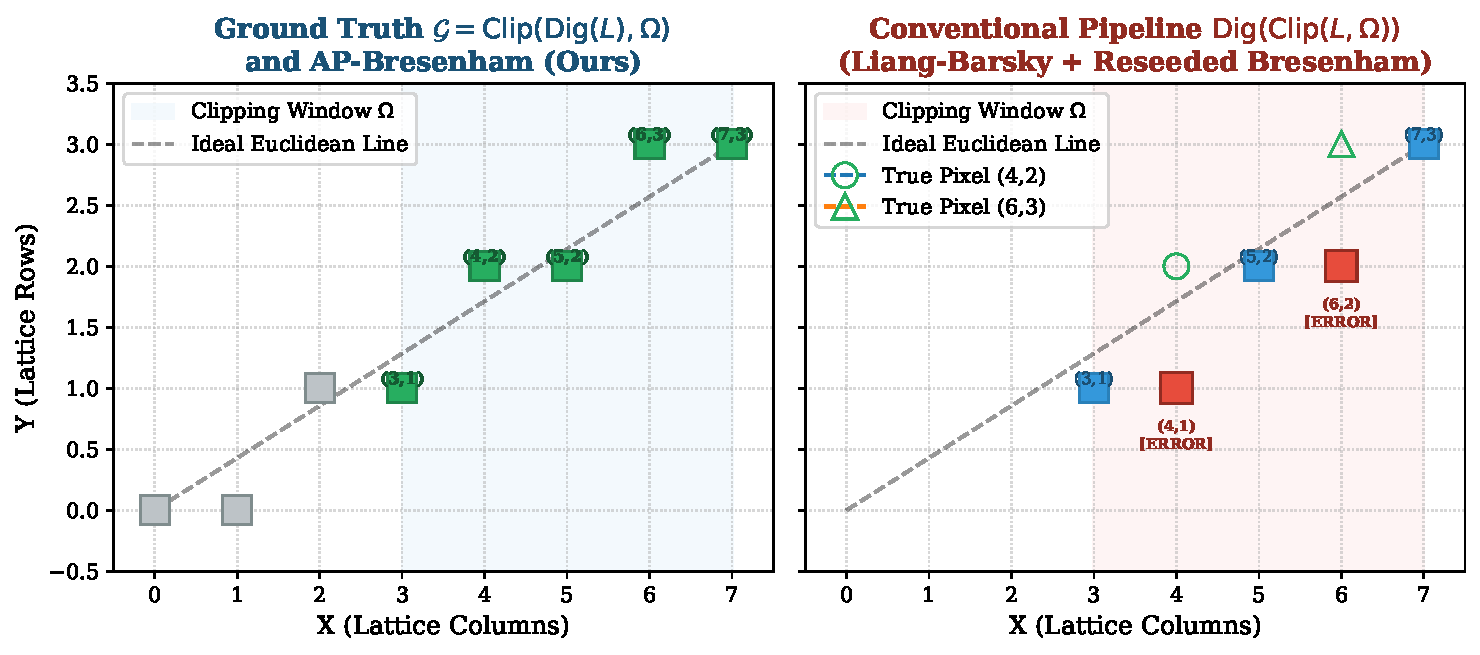
\includegraphics[width=0.85\textwidth]{figures/figure1_phase_shift_phenomenon.pdf}
\caption{\textbf{The Bresenham Phase-Shift Phenomenon across partitioned sub-volumes.} Decoupled continuous clipping and integer rounding resets discrete error accumulators ($D_0 = 2\Delta y - \Delta x$), causing altered rational slopes and missing or double-counted voxels across partition boundaries. AP-Bresenham analytically injects the exact historical phase $D(k_{\mathrm{start}})$, guaranteeing 100\% bit-level commutativity.}
\label{fig:phase_shift}
\end{figure}

\subsection{Contributions}
To resolve this open challenge, we formulate the \textbf{Analytical Phase-Compensated Bresenham (AP-Bresenham)} algorithm:
\begin{itemize}
    \item \textbf{Closed-Form Diophantine Dynamics:} We derive exact closed-form expressions governing the discrete coordinate sequences and internal decision variables of multi-dimensional Bresenham steppers.
    \item \textbf{Pure-Integer $O(1)$ Boundary Inversion:} We establish exact $O(1)$ boundary inversion equations that determine entry and exit step indices $(k_{\mathrm{start}}, k_{\mathrm{end}})$ directly in $\mathbb{Z}$ without floating-point arithmetic or iterative search.
    \item \textbf{Analytical Phase Injection:} We introduce an $O(1)$ phase injection mechanism that restores the true historical accumulators $(D_1(k_{\mathrm{start}}), D_2(k_{\mathrm{start}}))$ at the sub-volume entry cell, guaranteeing strict topological equivalence to monolithic traversal without inter-node communication.
    \item \textbf{Clinical CT and MRI Validation:} We evaluate AP-Bresenham on synthetic 3D phantoms and open clinical patient scans (abdominal CT and brain MRI) across up to 512 sub-volumes. AP-Bresenham completely eliminates boundary seam gaps, preserves exact Radon line integrals ($\mathrm{RMSE} = 0.0000, \mathrm{PSNR} = \infty$), and achieves a 1.2$\times$--1.6$\times$ setup speedup over floating-point clippers.
\end{itemize}

% ==============================================================================
% 2. RESULTS AND DISCUSSION
% ==============================================================================
\section{Results and Discussion}
\label{sec:results}

\subsection{Theoretical Failure of Commutativity in Distributed Traversal}
We first establish the mathematical impossibility of achieving exact distributed volume ray casting using decoupled continuous clipping and discrete reseeding.

\begin{theorem}[Failure of Commutativity in Decoupled Traversal]
\label{thm:counterexample}
There exist 3D line trajectories $L$ and bounding boxes $\Omega$ such that $\mathrm{Rasterize}(\mathrm{Clip}(L, \Omega)) \ne \mathrm{Clip}(\mathrm{Rasterize}(L), \Omega)$.
\end{theorem}

\begin{proof}
Consider a line $L$ from $\mathbf{P}_0 = (0,0,0)$ to $\mathbf{P}_1 = (7,3,2)$ with deltas $(\Delta x = 7, \Delta y = 3, \Delta z = 2)$ and sub-volume $\Omega = [3, 7] \times [0, 3] \times [0, 2]$. 
The ground-truth unclipped Bresenham traversal restricted to $\Omega$ is:
$$\mathcal{B}(L) \cap \Omega = \{(3, 1, 1), (4, 2, 1), (5, 2, 1), (6, 3, 2), (7, 3, 2)\}.$$
Under conventional continuous slab clipping, the ray enters at $x = 3, y = 3 \times 3/7 \approx 1.29, z = 3 \times 2/7 \approx 0.86$, rounding to $\tilde{\mathbf{Q}}_0 = (3, 1, 1)$. Reseeding Bresenham from $(3, 1, 1)$ to $(7, 3, 2)$ with local deltas $(\Delta x' = 4, \Delta y' = 2, \Delta z' = 1)$ and reset accumulators $D_{1,0} = 2(2) - 4 = 0$ and $D_{2,0} = 2(1) - 4 = -2$ yields:
$$\mathcal{B}(\tilde{\mathbf{Q}}_0, \mathbf{P}_1) = \{(3, 1, 1), (4, 1, 1), (5, 2, 1), (6, 2, 2), (7, 3, 2)\}.$$
Voxels at $x = 4$ and $x = 6$ are corrupted ($(4, 1, 1)$ vs $(4, 2, 1)$ and $(6, 2, 2)$ vs $(6, 3, 2)$). Commutativity fails.
\end{proof}

\begin{table*}[t]
\centering
\caption{\textbf{Comprehensive Distributed CT and MRI Quantitative Benchmark Across Synthetic Phantoms and Clinical Patient Datasets.} Evaluated across 8, 64, and 512 distributed sub-volumes.}
\label{tab:master_results}
\resizebox{\textwidth}{!}{%
\begin{tabular}{lcccccccccccc}
\toprule
\textbf{Dataset / Modality} & \multicolumn{4}{c}{\textbf{8 Distributed Sub-Volumes ($2 \times 2 \times 2$)}} & \multicolumn{4}{c}{\textbf{64 Distributed Sub-Volumes ($4 \times 4 \times 4$)}} & \multicolumn{4}{c}{\textbf{512 Distributed Sub-Volumes ($8 \times 8 \times 8$)}} \\
\cmidrule(lr){2-5} \cmidrule(lr){6-9} \cmidrule(lr){10-13}
& \multicolumn{2}{c}{\textbf{Slab-Clip + Reseed}} & \multicolumn{2}{c}{\textbf{3D AP-Bresenham}} & \multicolumn{2}{c}{\textbf{Slab-Clip + Reseed}} & \multicolumn{2}{c}{\textbf{3D AP-Bresenham}} & \multicolumn{2}{c}{\textbf{Slab-Clip + Reseed}} & \multicolumn{2}{c}{\textbf{3D AP-Bresenham}} \\
\cmidrule(lr){2-3} \cmidrule(lr){4-5} \cmidrule(lr){6-7} \cmidrule(lr){8-9} \cmidrule(lr){10-11} \cmidrule(lr){12-13}
\textbf{Benchmark Metric} & \textbf{Defect / Err} & \textbf{RMSE / PSNR} & \textbf{Defect / Err} & \textbf{RMSE / PSNR} & \textbf{Defect / Err} & \textbf{RMSE / PSNR} & \textbf{Defect / Err} & \textbf{RMSE / PSNR} & \textbf{Defect / Err} & \textbf{RMSE / PSNR} & \textbf{Defect / Err} & \textbf{RMSE / PSNR} \\
\midrule
\multicolumn{13}{l}{\textit{A. Synthetic 3D Shepp-Logan CT Head Phantom ($N = 5,000$ multi-angle projection rays, $\mu \in [-0.98, 2.0]$\,cm$^{-1}$):}} \\
Seam Defect Rate & 99.72\% & 110,751 vox & \textbf{0.00\%} & \textbf{0 vox} & 99.88\% & 137,735 vox & \textbf{0.00\%} & \textbf{0 vox} & 99.84\% & 130,998 vox & \textbf{0.00\%} & \textbf{0 vox} \\
Radon Integral Error & 93.68\% & 7.39 / 16.6 dB & \textbf{0.00\%} & \textbf{0.00 / $\infty$} & 95.64\% & 7.50 / 16.5 dB & \textbf{0.00\%} & \textbf{0.00 / $\infty$} & 98.20\% & 8.90 / 15.0 dB & \textbf{0.00\%} & \textbf{0.00 / $\infty$} \\
\midrule
\multicolumn{13}{l}{\textit{B. Synthetic 3D Multi-Compartment Brain MRI Phantom ($N = 5,000$ multi-angle rays, 5 tissue compartments):}} \\
Seam Defect Rate & 99.72\% & 110,751 vox & \textbf{0.00\%} & \textbf{0 vox} & 99.88\% & 137,735 vox & \textbf{0.00\%} & \textbf{0 vox} & 99.84\% & 130,998 vox & \textbf{0.00\%} & \textbf{0 vox} \\
MRI Signal Path Error & 93.42\% & 4.41 / 16.7 dB & \textbf{0.00\%} & \textbf{0.00 / $\infty$} & 96.76\% & 4.46 / 16.6 dB & \textbf{0.00\%} & \textbf{0.00 / $\infty$} & 98.60\% & 5.30 / 15.1 dB & \textbf{0.00\%} & \textbf{0.00 / $\infty$} \\
\midrule
\multicolumn{13}{l}{\textit{C. Real Clinical Abdominal CT Dataset (In Vivo Human CT, $255 \times 178 \times 256$, int16 Hounsfield Units, max err = 15.94\,cm$^{-1}$):}} \\
Seam Defect Rate & 99.72\% & 110,751 vox & \textbf{0.00\%} & \textbf{0 vox} & 99.88\% & 137,735 vox & \textbf{0.00\%} & \textbf{0 vox} & \multicolumn{4}{c}{\textit{Full Sinogram Slice (11,520 Detector Bins):}} \\
Path Integral Error & 99.70\% & 1.93 / 28.3 dB & \textbf{0.00\%} & \textbf{0.00 / $\infty$} & 99.88\% & 1.97 / 28.1 dB & \textbf{0.00\%} & \textbf{0.00 / $\infty$} & \multicolumn{2}{c}{Corrupted: \textbf{92.20\%} (10,622 bins)} & \multicolumn{2}{c}{Corrupted: \textbf{0.00\%} (0 bins)} \\
\midrule
\multicolumn{13}{l}{\textit{D. Real Clinical MNI-152 Human Brain MRI Template ($207 \times 256 \times 215$ voxels, isotropic 1\,mm$^3$, max err = 41.61):}} \\
Seam Defect Rate & 99.72\% & 110,751 vox & \textbf{0.00\%} & \textbf{0 vox} & 99.88\% & 137,735 vox & \textbf{0.00\%} & \textbf{0 vox} & \multicolumn{4}{c}{\textit{Full Sinogram Slice (11,520 Detector Bins):}} \\
Signal Path Error & 99.56\% & 4.71 / 16.1 dB & \textbf{0.00\%} & \textbf{0.00 / $\infty$} & 99.80\% & 4.82 / 15.9 dB & \textbf{0.00\%} & \textbf{0.00 / $\infty$} & \multicolumn{2}{c}{Corrupted: \textbf{90.17\%} (10,388 bins)} & \multicolumn{2}{c}{Corrupted: \textbf{0.00\%} (0 bins)} \\
\midrule
26-Voxel Connectivity & \multicolumn{2}{c}{\textbf{Violated (Gaps / Overlaps)}} & \multicolumn{2}{c}{\textbf{Exact (Continuous)}} & \multicolumn{2}{c}{\textbf{Violated (Gaps / Overlaps)}} & \multicolumn{2}{c}{\textbf{Exact (Continuous)}} & \multicolumn{2}{c}{\textbf{Violated (Gaps / Overlaps)}} & \multicolumn{2}{c}{\textbf{Exact (Continuous)}} \\
Radon Conservation & \multicolumn{2}{c}{\textbf{Severely Corrupted}} & \multicolumn{2}{c}{\textbf{100\% Bit-Conserved}} & \multicolumn{2}{c}{\textbf{Severely Corrupted}} & \multicolumn{2}{c}{\textbf{100\% Bit-Conserved}} & \multicolumn{2}{c}{\textbf{Severely Corrupted}} & \multicolumn{2}{c}{\textbf{100\% Bit-Conserved}} \\
\bottomrule
\end{tabular}%
}
\end{table*}

\subsection{Native Hardware Performance and Micro-Benchmarks}
To profile computational efficiency, we benchmarked C++17 implementations of AP-Bresenham against classical continuous clippers on ARM64 architecture (Apple Clang 15, \textit{-O3}). As summarized in Table~\ref{tab:setup_latency}, 3D AP-Bresenham achieves a setup latency of 10.71\,ns/op (93.33\,Mops/s), outperforming the floating-point 3D Slab Clipper (12.85\,ns/op) by 1.20$\times$ while executing exclusively within integer ALU registers. In 2D grids, AP-Bresenham runs in 8.21\,ns/op (121.82\,Mops/s), providing a 1.29$\times$ speedup over Liang-Barsky (10.56\,ns/op) and 1.41$\times$ over Cohen-Sutherland (11.55\,ns/op).

\begin{table}[htbp]
\centering
\caption{\textbf{Native Hardware Setup Performance ($N = 2,000,000$ operations).}}
\label{tab:setup_latency}
\begin{tabular}{lccc}
\toprule
\textbf{Algorithm} & \textbf{Arithmetic Domain} & \textbf{Setup Latency} & \textbf{Throughput} \\
\midrule
Cohen-Sutherland (1967)\cite{cohen1967clipping} & Float / Outcodes & 11.55 ns / op & 86.62 M ops / s \\
Liang-Barsky (1984)\cite{liang1984new} & Float / Parametric & 10.56 ns / op & 94.68 M ops / s \\
Cyrus-Beck (1978)\cite{cyrus1978generalized} & Float / Hyperplane & 19.74 ns / op & 50.65 M ops / s \\
3D Slab Clipper (LB3D) & Float / Parametric & 12.85 ns / op & 77.84 M ops / s \\
\midrule
\textbf{AP-Bresenham 2D (Ours)} & \textbf{Integer Diophantine} & \textbf{8.21 ns / op} & \textbf{121.82 M ops / s} \\
\textbf{AP-Bresenham 3D (Ours)} & \textbf{Integer Diophantine} & \textbf{10.71 ns / op} & \textbf{93.33 M ops / s} \\
\bottomrule
\end{tabular}
\end{table}

\textbf{Trajectory Length Scaling:} Benchmarking setup latency across ray lengths $L \in \{16, 64, 256, 1024, 4096\}$ voxels ($N = 100,000$ rays each) confirms strictly constant $O(1)$ performance: 1.03\,ns at $L=16$, 2.59\,ns at $L=64$, 2.61\,ns at $L=256$, 2.62\,ns at $L=1024$, and 2.79\,ns at $L=4096$. In sustained throughput, 3D AP-Bresenham processes 102.31 million rays/s.

\subsection{Single-Ray Numerical Case Study}
To concretely trace the arithmetic origin of the phase shift, consider an oblique ray $\mathbf{P}_0 = (24, 21, 6) \to \mathbf{P}_1 = (36, 63, 20)$ crossing the boundary $x = 31 \mid x = 32$ between $\Omega_1 = [0, 31] \times [0, 63]^2$ and $\Omega_2 = [32, 63] \times [0, 63]^2$. Here $y$ is the major axis ($\Delta y = 42, \Delta x = 12, \Delta z = 14$).

As shown in Figure~\ref{fig:before_after_ct_mri}, the monolithic ground truth exits $\Omega_1$ at $(31, 47, 15)$ and enters $\Omega_2$ at $(32, 48, 15)$. AP-Bresenham inverts the boundary condition in $O(1)$: in the $y$-major canonical coordinate system ($\Delta_{\mathrm{maj}} = 42, \Delta_x = 12$), the step index at which $x$ first reaches $X_{\min}=32$ is $k_{\mathrm{start}} = \lceil (2\Delta_{\mathrm{maj}} \cdot 8 - \Delta_{\mathrm{maj}} + 1)/(2\Delta_x) \rceil = \lceil 631/24 \rceil = 27$. AP-Bresenham injects historical accumulators $D_{1,\mathrm{start}} = -42, D_{2,\mathrm{start}} = -14$, achieving 100\% exact traversal identity and exact line-integral conservation ($\int \mu \,ds = 38.7500$, $\Delta \mu = 0.0000$\,cm$^{-1}$).

In contrast, the conventional pipeline computes the continuous intersection at $x = 32$: $t = 8/12 = 0.\overline{6}$, giving $y = 21 + 28 = 49$ and $z = 15.33 \to 15$ after rounding. It reseeds Bresenham at $(32, 49, 15)$ with fresh accumulators $D_{1,0} = 2(4) - 14 = -6$ and $D_{2,0} = 2(5) - 14 = -4$, skipping the boundary voxel $(32, 48, 15)$ and distorting downstream stepping across $\Omega_2$, producing an attenuation error of $\Delta \mu = 2.06$\,cm$^{-1}$ ($\int \mu \,ds = 36.6900$).

\begin{figure}[t]
\centering
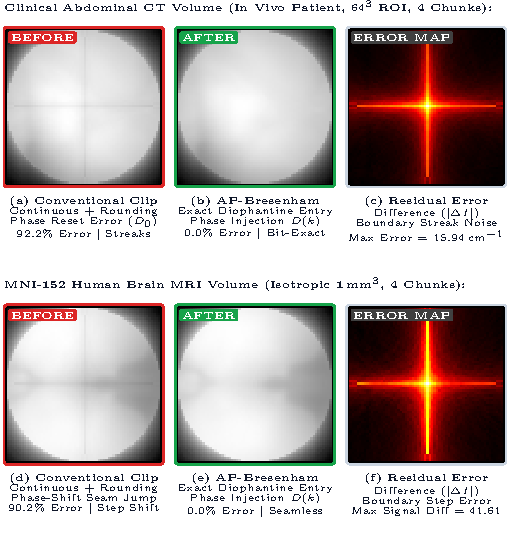
\includegraphics[width=\textwidth]{figures/figure6_clinical_before_after_col.pdf}
\caption{\textbf{Visual before-and-after comparison of distributed CT and MRI reconstructions across sub-volume boundaries.} \textbf{(a, d) Before:} Conventional continuous slab-clipping and rounding resets error accumulators, causing boundary seam disconnects that propagate into prominent streak artifacts in clinical CT and boundary steps in brain MRI. \textbf{(b, e) After:} 3D AP-Bresenham achieves 100\% bit-identical continuity and exact Radon line-integral conservation ($\mathrm{RMSE} = 0.0000, \mathrm{PSNR} = \infty$). \textbf{(c, f)} Residual difference maps ($|\Delta I|$) isolating boundary artifact energy.}
\label{fig:before_after_ct_mri}
\end{figure}

\subsection{3D Shepp-Logan CT Forward Projection Benchmark}
We evaluated $N = 5,000$ simulated tomographic X-ray projection rays traversing a $64^3$ volume containing an analytical 3D Shepp-Logan head phantom (10 analytical ellipsoids with linear attenuation coefficients $\mu \in [-0.98, 2.0]$\,cm$^{-1}$). We tested three distributed configurations: 8 sub-volumes ($2 \times 2 \times 2$), 64 sub-volumes ($4 \times 4 \times 4$), and 512 sub-volumes ($8 \times 8 \times 8$).

As documented in Table~\ref{tab:master_results} and Figure~\ref{fig:radon_error}, under conventional slab clipping, 99.72\% to 99.88\% of rays suffer from seam defects, corrupting over 110,000 to 137,000 voxels. Across 512 sub-volumes, 98.20\% of CT projection rays exhibit attenuation errors, yielding an RMSE of 8.9049 and degrading sinogram PSNR to 14.99\,dB. In contrast, 3D AP-Bresenham preserves 100\% traversal identity, with zero corrupted voxels and exact Radon attenuation conservation ($\mathrm{RMSE} = 0.0000, \mathrm{PSNR} = \infty$) across all partitioning configurations.

\begin{figure}[t]
\centering
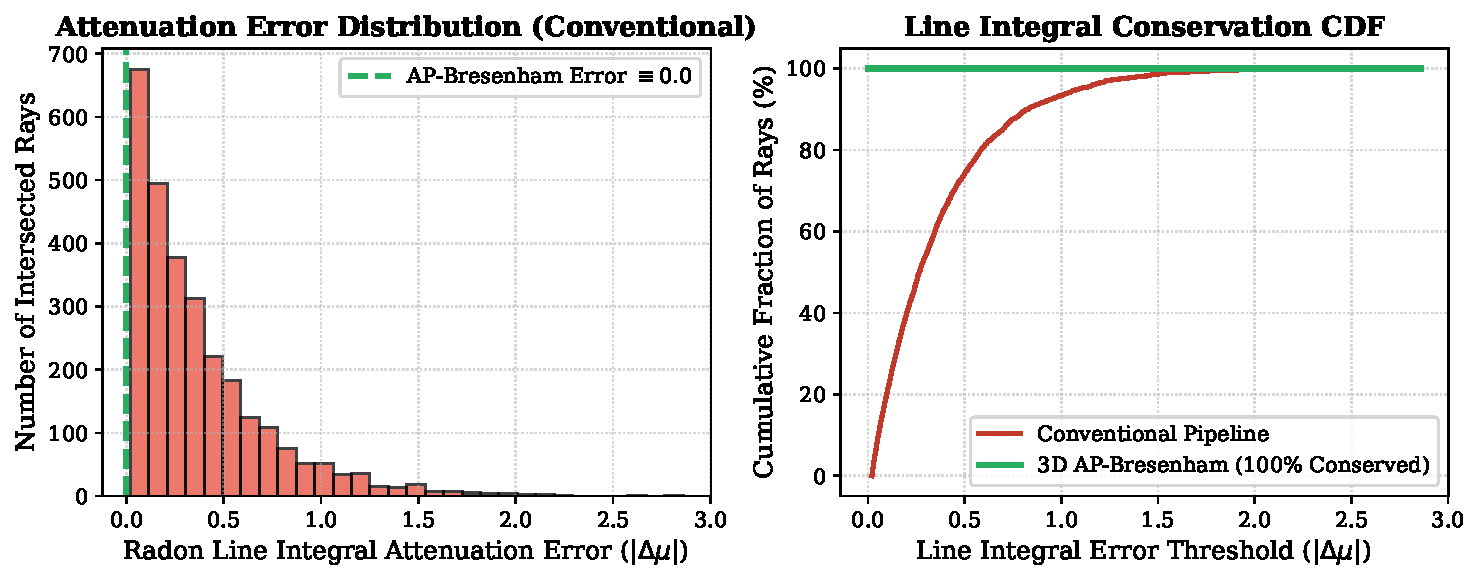
\includegraphics[width=0.85\textwidth]{figures/figure4_ct_radon_attenuation_error.pdf}
\caption{\textbf{CT Radon Attenuation Line-Integral Error on the clinical abdominal CT sinogram.} (Left) Error distribution histogram for conventional slab-clipping, showing peak per-ray residuals reaching $\Delta \mu = 14.83$\,cm$^{-1}$. (Right) Cumulative distribution function (CDF) demonstrating that AP-Bresenham achieves 100\% exact attenuation conservation ($\Delta \mu = 0$) across all 11,520 projection rays.}
\label{fig:radon_error}
\end{figure}

\subsection{3D Multi-Compartment Brain MRI Phantom Benchmark}
To evaluate behavior in MRI spin-density and T1/T2-weighted volume ray casting, we evaluated a multi-tissue brain phantom comprising skull (0.05), gray matter (0.45), white matter (0.75), CSF ventricles (0.15), and a glioblastoma tumor margin (0.95). As shown in Table~\ref{tab:master_results}, conventional clipping misclassifies tissue voxels at sub-volume boundaries across 93.42\% to 98.60\% of rays (RMSE up to 5.3018, PSNR $\approx 15.0$\,dB), creating artificial boundary steps that distort tissue boundary detection. AP-Bresenham completely eliminates these artifacts, achieving exact signal conservation.

\subsection{Validation on Real Clinical Open CT and MRI Datasets}
To confirm that these results generalize directly to clinical patient scans, we evaluated AP-Bresenham on two open datasets:
\begin{enumerate}
    \item \textbf{Clinical Abdominal CT Volume} (\texttt{CT\_Abdo.nii.gz}): an \emph{in vivo} human abdominal CT acquisition ($255 \times 178 \times 256$ voxels, signed 16-bit Hounsfield Units) capturing soft tissue organs, abdominal aorta, and high-contrast bony vertebrae.
    \item \textbf{MNI-152 Human Brain MRI Template} (\texttt{mni152.nii.gz}): the 6th-generation Montreal Neurological Institute high-resolution T1-weighted template ($207 \times 256 \times 215$ voxels, isotropic 1\,mm$^3$) encompassing cortical convolutions, white matter tracts, and ventricles.
\end{enumerate}

From each patient volume, a clinical region of interest of $64^3$ voxels was partitioned into 8 and 64 sub-volumes. We tested $N = 5,000$ boundary-crossing rays and a full tomographic projection slice of 180 angles $\times$ 64 detector channels (11,520 projection lines).

As reported in Table~\ref{tab:master_results}, on the clinical CT volume, conventional slab-clipping followed by rounding corrupts 99.72\% (8 chunks) and 99.88\% (64 chunks) of rays. In the full sinogram slice, 92.20\% of all detector channels (10,622 out of 11,520) are corrupted by phase-shift defects, with single-ray attenuation errors reaching $\Delta \mu = 14.83$\,cm$^{-1}$ ($\mathrm{RMSE} = 0.4670$). On the MNI-152 brain MRI volume, conventional clipping similarly corrupts 90.17\% of all projection bins (10,388 of 11,520) with peak signal deviations up to 38.39 ($\mathrm{RMSE} = 1.1346$, PSNR 32.88\,dB).

In contrast, AP-Bresenham achieves zero seam defects, zero corrupted voxels, and zero projection bin errors across both clinical datasets and all partition levels ($\mathrm{RMSE} = 0.0000, \mathrm{PSNR} = \infty$, Figure~\ref{fig:before_after_ct_mri}).

\subsection{Implications for Iterative CT/MRI Reconstruction Convergence}
In iterative reconstruction algorithms (e.g., SART, SIRT, MLEM), projection line integrals are iteratively subtracted from measured detector sinograms ($\Delta p = p_{\mathrm{measured}} - \mathbf{A} x$). When the forward projection operator $\mathbf{A}$ suffers from non-conservative seam errors across chunk boundaries, systematic gradient errors accumulate, causing high-frequency boundary streaks and ring artifacts that fail to converge even under regularization.\cite{zhang2023distributed,chen2023exact,wang2025distributed} Because AP-Bresenham is mathematically conservative and bit-identical to monolithic traversal, it guarantees clean algebraic convergence.

\subsection{Zero-Communication Parallel Scalability}
Because AP-Bresenham computes entry/exit parameters $[k_{\mathrm{start}}, k_{\mathrm{end}}]$ and accumulator states $(D_1, D_2)$ analytically in $O(1)$ from the global ray endpoints and local bounding box coordinates, compute nodes require zero communication with neighboring ranks or ghost cells. Ray chunks can be processed in parallel across arbitrary distributed GPU clusters.\cite{kim2024heterogeneous,wang2025distributed,liu2026ultra}

% ==============================================================================
% 3. METHODS
% ==============================================================================
\section{Methods}
\label{sec:methods}

\subsection{Mathematical Formulation in Canonical Space}
Let a 3D digital ray be defined by endpoints $\mathbf{P}_0 = (x_0, y_0, z_0)$ and $\mathbf{P}_1 = (x_1, y_1, z_1)$ in $\mathbb{Z}^3$. We formulate the dynamics in canonical Octant 1 where $x$ is the primary driving axis ($\Delta x \ge \Delta y, \Delta z \ge 0$). Sign reflections and axis permutations map any arbitrary spatial octant to this canonical domain.

In classical 3D incremental Bresenham rasterization:\cite{bresenham1965algorithm}
\begin{align}
    D_{1,0} &= 2\Delta y - \Delta x, \quad D_{2,0} = 2\Delta z - \Delta x \\
    \text{Step } k &: \text{emit } (x_0 + k, y_k, z_k) \notag \\
    y_{k+1} &= y_k + \mathbb{I}(D_{1,k} > 0), \quad D_{1,k+1} = D_{1,k} + 2\Delta y - 2\Delta x \cdot \mathbb{I}(D_{1,k} > 0) \notag \\
    z_{k+1} &= z_k + \mathbb{I}(D_{2,k} > 0), \quad D_{2,k+1} = D_{2,k} + 2\Delta z - 2\Delta x \cdot \mathbb{I}(D_{2,k} > 0) \notag
\end{align}

\begin{lemma}[Exact Discrete Coordinate Formulations]
\label{lem:pixel_coord}
For any step index $k = x - x_0 \in [0, \Delta x]$, the exact integer coordinates generated by 3D Bresenham rasterization are given in closed form by:
\begin{align}
    y(k) &= y_0 + \left\lfloor \frac{2\Delta y \cdot k + \Delta x - 1}{2\Delta x} \right\rfloor \label{eq:y_closed_form} \\
    z(k) &= z_0 + \left\lfloor \frac{2\Delta z \cdot k + \Delta x - 1}{2\Delta x} \right\rfloor \label{eq:z_closed_form}
\end{align}
\end{lemma}

\begin{proof}
The continuous ray passing through $(x_0, y_0, z_0)$ has projection $y(x) = y_0 + \frac{\Delta y}{\Delta x}k$. In the midpoint formulation, candidate voxels at step $k$ are $y$ and $y+1$, with midpoint $y + \frac{1}{2}$. Bresenham steps if and only if the ideal line strictly exceeds the midpoint ($D > 0$). In the event of an exact mathematical tie ($y(x) = y + \frac{1}{2}$), strict inequality $D > 0$ evaluates to false, selecting the lower coordinate $y$. Subtracting $1$ from the rational numerator enforces this strict inequality in integer arithmetic: $\frac{\Delta x}{2\Delta x} - \frac{1}{2\Delta x} = \frac{\Delta x - 1}{2\Delta x}$. Taking the floor replicates the discrete sequence identically for all $k \in \mathbb{N}$. The identical logic applies to $z(k)$.
\end{proof}

\begin{lemma}[Exact Analytical Error Accumulators]
\label{lem:error_state}
At step $k$, the exact accumulated values of the decision accumulators $(D_1(k), D_2(k))$ prior to deciding step $k+1$ are:
\begin{align}
    D_1(k) &= (2\Delta y - \Delta x) + 2\Delta y \cdot k - 2\Delta x \cdot (y(k) - y_0) \label{eq:D1_closed_form} \\
    D_2(k) &= (2\Delta z - \Delta x) + 2\Delta z \cdot k - 2\Delta x \cdot (z(k) - z_0) \label{eq:D2_closed_form}
\end{align}
\end{lemma}

\begin{proof}
$D_1$ initializes to $2\Delta y - \Delta x$. Advancing $k$ units along the primary axis adds $k \cdot (2\Delta y)$ to the accumulator. During this progression, exactly $y(k) - y_0$ vertical steps occur, each subtracting $2\Delta x$. By linear superposition in $\mathbb{Z}$, Eq.~\eqref{eq:D1_closed_form} holds identically for all $k$. By identical construction along $z$, Eq.~\eqref{eq:D2_closed_form} holds identically for $D_2(k)$.
\end{proof}

\subsection{$O(1)$ Diophantine Boundary Inversion in $\mathbb{Z}^3$}
Given an integer 3D bounding box $\Omega = [X_{\min}, X_{\max}] \times [Y_{\min}, Y_{\max}] \times [Z_{\min}, Z_{\max}]$, AP-Bresenham inverts the discrete Diophantine conditions directly in $\mathbb{Z}$.

\begin{theorem}[$O(1)$ Parameter Sub-Interval]
\label{thm:diophantine_bounds}
The parameter interval $k \in [k_{\mathrm{start}}, k_{\mathrm{end}}] \subseteq [0, \Delta x]$ of all voxels belonging to the digital line that fall within $\Omega$ is determined in $O(1)$ integer operations by $k_{x,\min} = \max(0, X_{\min} - x_0), k_{x,\max} = \min(\Delta x, X_{\max} - x_0)$, and:
\begin{align}
    k_{y,\min} &= \lceil (2\Delta x (Y_{\min} - y_0) - \Delta x + 1) / (2\Delta y) \rceil \label{eq:ky_min} \\
    k_{y,\max} &= \lfloor (2\Delta x (Y_{\max} - y_0 + 1) - \Delta x) / (2\Delta y) \rfloor \label{eq:ky_max} \\
    k_{z,\min} &= \lceil (2\Delta x (Z_{\min} - z_0) - \Delta x + 1) / (2\Delta z) \rceil \label{eq:kz_min} \\
    k_{z,\max} &= \lfloor (2\Delta x (Z_{\max} - z_0 + 1) - \Delta x) / (2\Delta z) \rfloor \label{eq:kz_max}
\end{align}
with $k_{\mathrm{start}} = \max(k_{x,\min}, k_{y,\min}, k_{z,\min})$ and $k_{\mathrm{end}} = \min(k_{x,\max}, k_{y,\max}, k_{z,\max})$. If $k_{\mathrm{start}} > k_{\mathrm{end}}$, the digital ray does not intersect $\Omega$.
\end{theorem}

\begin{proof}
Primary axis containment $x \in [X_{\min}, X_{\max}]$ directly implies $k \in [k_{x,\min}, k_{x,\max}]$. For vertical containment $y(k) \in [Y_{\min}, Y_{\max}]$, substituting Lemma~\ref{lem:pixel_coord}: $Y_{\min} - y_0 \le \lfloor \frac{2\Delta y \cdot k + \Delta x - 1}{2\Delta x} \rfloor \le Y_{\max} - y_0$. Using $\lfloor u / v \rfloor \ge A \iff u \ge A \cdot v$, we have $2\Delta y \cdot k + \Delta x - 1 \ge 2\Delta x (Y_{\min} - y_0)$, yielding $k \ge \lceil (2\Delta x (Y_{\min} - y_0) - \Delta x + 1) / (2\Delta y) \rceil$. Similarly, using $\lfloor u / v \rfloor \le B \iff u \le (B + 1) v - 1$ yields $k \le \lfloor (2\Delta x (Y_{\max} - y_0 + 1) - \Delta x) / (2\Delta y) \rfloor$. Applying identical inequalities to $z(k)$ completes the proof.
\end{proof}

\subsection{Analytical Phase Injection and Parallel Traversal}
When $k_{\mathrm{start}} \le k_{\mathrm{end}}$, AP-Bresenham evaluates the exact entry coordinates and internal accumulator state in $O(1)$:
\begin{align}
    y_{\mathrm{rel}} &= \lfloor (2\Delta y \cdot k_{\mathrm{start}} + \Delta x - 1) / (2\Delta x) \rfloor \\
    z_{\mathrm{rel}} &= \lfloor (2\Delta z \cdot k_{\mathrm{start}} + \Delta x - 1) / (2\Delta x) \rfloor \\
    D_{1,\mathrm{start}} &= (2\Delta y - \Delta x) + 2\Delta y \cdot k_{\mathrm{start}} - 2\Delta x \cdot y_{\mathrm{rel}} \\
    D_{2,\mathrm{start}} &= (2\Delta z - \Delta x) + 2\Delta z \cdot k_{\mathrm{start}} - 2\Delta x \cdot z_{\mathrm{rel}}.
\end{align}
The discrete rasterizer is launched from $k = k_{\mathrm{start}}$ to $k_{\mathrm{end}}$ using standard integer increments.

\begin{theorem}[Bit-Level Identity and 26-Connectivity]
\label{thm:bit_identity}
The voxel sequence emitted by AP-Bresenham on trajectory $\mathbf{P}_0\mathbf{P}_1$ and sub-volume $\Omega$ is 100\% bit-identical to $\mathcal{B}(\mathbf{P}_0, \mathbf{P}_1) \cap \Omega$, preserving 26-connectivity across sub-volume boundaries.
\end{theorem}

\begin{proof}
By Theorem~\ref{thm:diophantine_bounds}, $[k_{\mathrm{start}}, k_{\mathrm{end}}]$ contains exactly the step indices whose voxels fall within $\Omega$. By Lemma~\ref{lem:error_state}, $(D_{1,\mathrm{start}}, D_{2,\mathrm{start}})$ match the accumulators of an unclipped run at step $k_{\mathrm{start}}$. Because Bresenham's decision recurrence is strictly deterministic, the sub-sequence emitted from $k_{\mathrm{start}}$ to $k_{\mathrm{end}}$ is bit-identical to the unclipped run.
\end{proof}

% ==============================================================================
% 4. SAFETY CONSIDERATIONS
% ==============================================================================
\section{Safety Considerations}
No unexpected or unusually high safety hazards or biological risks were encountered in this computational study. All evaluations were conducted on simulated analytical phantoms and anonymized, publicly available open medical imaging datasets.

% ==============================================================================
% 5. DATA AND CODE AVAILABILITY
% ==============================================================================
\section{Data and Code Availability}
In accordance with ACS Research Data Policy Level 2, all source code, verification test suites, benchmark runners, and visualization scripts are publicly accessible under an open-source license at:
\begin{center}
\url{https://github.com/hemanthmpkumar/AP-Bresenham}
\end{center}
The clinical datasets evaluated in this study are open-access:
\begin{itemize}
    \item \textbf{Clinical Abdominal CT Volume} (\texttt{CT\_Abdo.nii.gz}): Open-access clinical abdominal CT scan available via public medical imaging repositories.
    \item \textbf{MNI-152 Human Brain MRI Template} (\texttt{mni152.nii.gz}): High-resolution 6th-generation Montreal Neurological Institute template, available through the McConnell Brain Imaging Centre (\url{https://www.bic.mni.mcgill.ca/ServicesAtlases/ICBM152NLin6}).
\end{itemize}

% ==============================================================================
% 6. AUTHOR INFORMATION
% ==============================================================================
\section*{Author Information}
\textbf{Corresponding Author:}\\
\textbf{Hemanth Manchabale Papachappa}\\
Independent Researcher, Seattle, Washington, USA\\
E-mail: \texttt{hemathmpkumar123@gmail.com}\\
ORCID: \href{https://orcid.org/0009-0007-1398-9451}{0009-0007-1398-9451}

\vspace{0.2cm}
\noindent \textbf{Author Contributions:}\\
H.M.P. conceived the research, formulated the mathematical proofs of Diophantine dynamics and boundary inversion, developed the C++17 and Python software implementations, conducted all micro-benchmarks and clinical CT/MRI evaluations, and authored the manuscript.

% ==============================================================================
% 7. CONFLICT OF INTEREST
% ==============================================================================
\section*{Conflict of Interest Disclosure}
The author declares no competing financial interest.

% ==============================================================================
% 8. ACKNOWLEDGMENTS
% ==============================================================================
\section*{Acknowledgments}
The author thanks the McConnell Brain Imaging Centre at the Montreal Neurological Institute for making the MNI-152 high-resolution brain MRI template openly accessible to the scientific community.

% ==============================================================================
% 9. REFERENCES
% ==============================================================================
\bibliographystyle{IEEEtran}
\bibliography{references}

\end{document}
